\documentclass[iop,apj,tighten]{emulateapj}
%\pdfoutput=1 %for arxiv submission to use pdf
\usepackage{apjfonts} %If missing fonts, comment out this or google apjfonts to download
\usepackage{amsmath,amstext}
\usepackage[breaklinks,colorlinks,citecolor=blue,linkcolor=magenta]{hyperref} 
\usepackage[all]{hypcap} %Links go to figures. This breaks deluxetables; use \capstartfalse \capstarttrue around deluxetables to fix it.

\renewcommand*{\sectionautorefname}{Section} %for \autoref
\renewcommand*{\subsectionautorefname}{Section} %for \autoref

\shorttitle{Galaxy Zoo: Illustris}
\shortauthors{Willett et al.}

\begin{document}

\title{Crowdsourced morphological classifications of Illustris synthetic galaxy images}
\author{K.W. Willett\altaffilmark{1} et al.}
\affil{$^1$University of Minnesota}

\begin{abstract}
Abstract.
\end{abstract}

\keywords{keywords}
\maketitle

\section{Science case}

Crowdsourced classifications of Illustris synthetic images \citep{sny15,tor15} using the Galaxy Zoo \citep{lin08,wil13} interface. 

\section{Data}

As of 15 Feb 2016, there have been 17,046 images classified in GZ-Illustris. 

The total Illustris sample has 110,256 images. That's from 6,891 unique galaxies using a mass-limited sample from the $z=0$ slice in the Illustris-1 simulation \citep{vog14a}. Each galaxy has 16 corresponding composite images --- 1~galaxy $\times$ 4~camera angles $\times$ 4~randomly-selected backgrounds. The total set of images is split into three groups:

\begin{itemize}

\item fixed\_mass (10,832~galaxies) --- I selected two narrow mass ranges (low and high) and then selected images with all camera angles and backgrounds within it. This is for analyzing the effect of viewing angle and background on morphological accuracy.
\item fixed\_view (6,214~galaxies) --- these span the full mass range of the sample, but with only 1~camera angle and background per galaxy. This is for doing an initial survey of the morphological distributions. The reason that this isn't 6,891 is because several hundred of the images were already classified in fixed\_mass.
\item full\_sample (93,210~galaxies) --- all the rest.

\end{itemize}
Both the fixed\_view and fixed\_mass samples have just been completed at 40~classifications each. Illustris is now paused, so the full\_sample doesn't have any classifications yet. 

\section{Analysis}

Figure~\ref{fig:piechart} shows a summary of the morphological demographics for the entire sample. 

\begin{figure*}
\centering
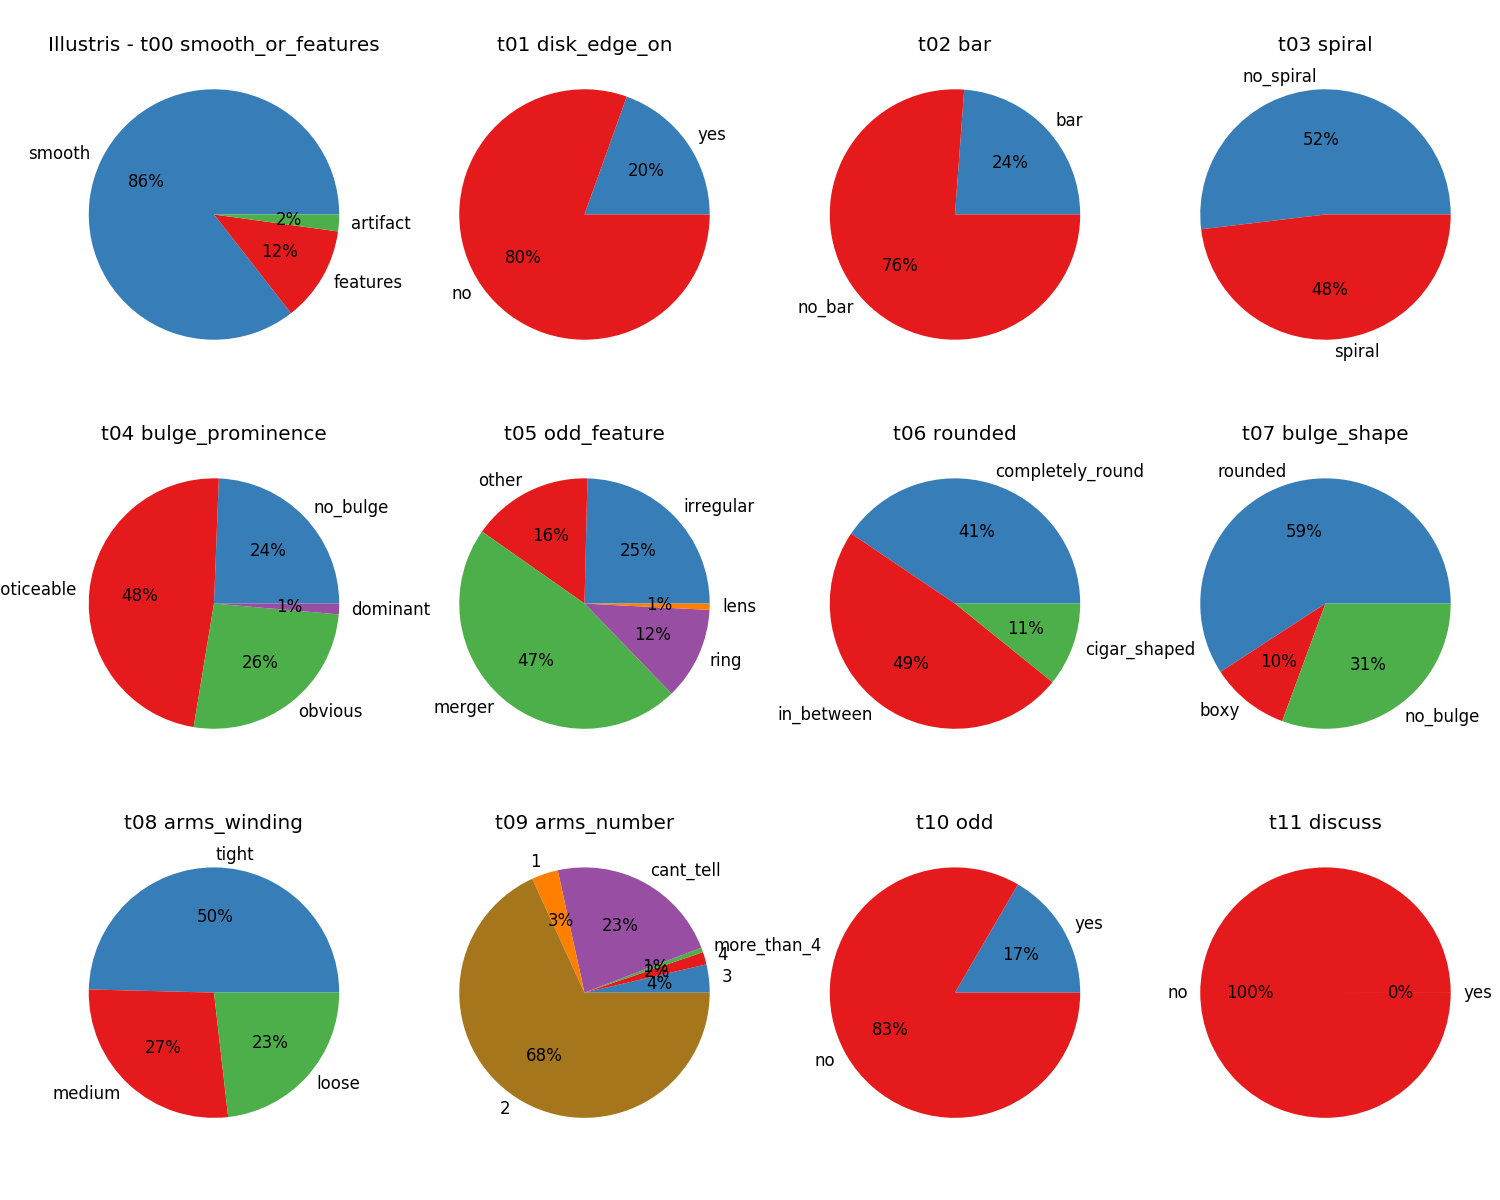
\includegraphics[width=160mm]{../plots/pie_illustris.png}
\caption{Distribution of the plurality morphological category for each task in GZ:Illustris. Labels show the percentage of each morphology only for those galaxies for which the question was reached in the hierarchical tree.\label{fig:piechart}}
\end{figure*}


\acknowledgments{
}

\bibliographystyle{yahapj}
\bibliography{kwrefs}

\end{document}
